\documentclass{article}

\usepackage{a4wide}
\usepackage{graphicx}
\usepackage{paralist}
\usepackage{hyperref}

\setlength{\parindent}{0em}
\setlength{\parskip}{1em}

\title{Project Information Security \\ Securing an online exam}
\author{Pieter De Baets, Gilles Jacobs, Jasper Van der Jeugt, Toon Willems}

\begin{document}

\maketitle
\tableofcontents

\newpage

\section{Introduction}

\section{Requirements and Architecture}

We chose to design a system with a central component, i.e. a server, to which
the different clients can connect. For users, it would appear that this central
server is their exam platform. This is not true however, as responsibilities and
software is distributed over all platform participants.

One disadvantage of this approach is that this server needs to be trusted to
some extent by the users, which we tried to limit as much as possible.

\subsection{Assumptions}

We need to assume that every user (students as well as professors) are
registered on this platform. These accounts can be created when a student
enrolls in the institute, or when a professor is employed.

The users of the platform should be able to verify that they are indeed
talking to the official platform instance, and not to some rogue machine posing
as the platform. This problem is mostly alleviated by using HTTPS and a trusted
cerficate for all communication.

% TODO: misschien wat specifieker zeggen wat HTTPS oplost?

We use an asymmetric encryption mechanism for many features, so we also need to
assume that each user has a keypair assigned. These keypairs can be created at
the same time as the accounts, with some option to reset a keypair when it has
been compromised. The platform only requires a user's public key, the private
key is

Ideally these keys are also signed by an official entitity so
that users can lookup and trust public keys found through a public key exchange.

\subsection{Functionality}

\subsubsection{Logging in}

Users (students and professors) should be able to log in to the application.
This means we need some kind of authentication: it is obvious that a student
should not be able to pose as a professor.

It is definitely possible to design a custom secure authentication solution.
However, given the setting, we chose for a more realistic option. Most large
organisations have an in-house authentication gateway which applications can
use. This way authentication can be organised securely across the whole
organisation without much effort to application developers.

\begin{figure}
\begin{center}
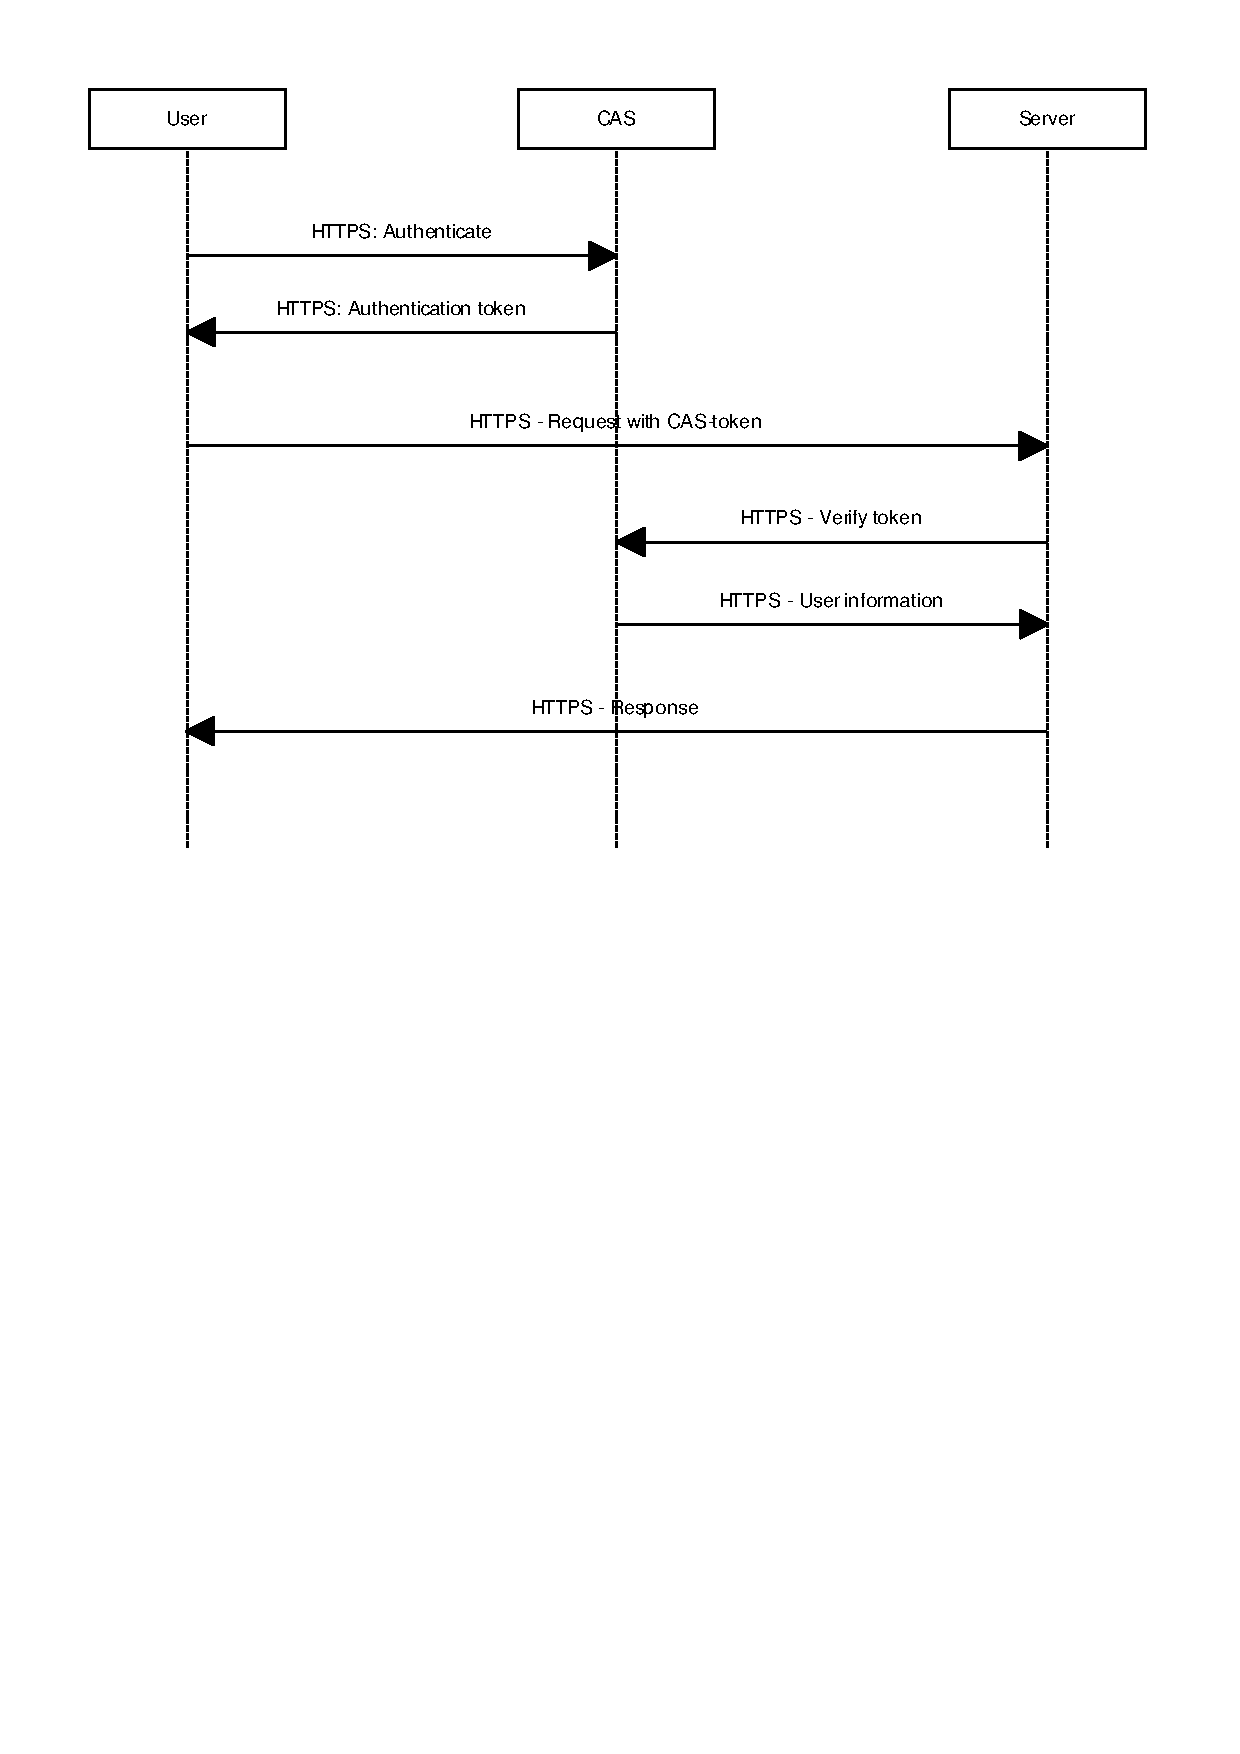
\includegraphics[width=0.75\textwidth]{images/login.pdf}
\caption{Messages exchanged when logging in}
\label{fig:login}
\end{center}
\end{figure}

For our proof-of-concept we integrated with Ghent University's Central
Authentication Server\footnote{\url{http://helpdesk.ugent.be/webhosting/en/cas.php}}
(CAS) which is an implementation of the publicly available CAS
protocol\footnote{\url{http://www.jasig.org/cas/protocol/}}. The basic
exchange of messages between user, CAS server and application server can be seen
in figure \ref{fig:login} and is summarized below.

\begin{enumerate}
\item The user has no active session on the exam server and is redirected
  to the authentication server (referencing the exam server as source).
\item The authentication server verifies the identify of the user. In our
  example this is a basic password authentication scheme (in which hopefully a
  secure hash of the password is used instead of a plaintext version), but more
  advanced options (e.g. smart cards, biometrics, ...) are possible as well.
\item When authentication has succeeded the authentication server generates
  a security token and returns the user to the exam server, carrying this token.
\item The exam server will then contact the authentication server and confirm
  the user's identify by using this token. The use of the token is strictly
  regulated to prevent abuse: only the requesting service can use it, it is only
  valid during a small timeframe and can only be used once.
\item Having received this information, the exam server can now start a local
  application session for the authenticated user.
\end{enumerate}

\subsubsection{Distributing exams}

The professor needs to be able to distribute an exam to the students. He first
uploads it to the central server, and selects a number of students. These
students can download it from there, at some point in time, also specified by
the professor.

Integrity is important here: we must ensure the students see the same exam that
the professor posted. Furthermore, only the selected students should be able to
see the exam, and we have to make sure they cannot view the exam before they are
allowed to.



\subsection{Expected attacks}

How will attackers try to compromise our system? Why will they fail?

\subsection{Limitations}

In what ways is our system not protected? What do we need to trust?

\section{Practical considerations}

Is it practically feasible to lock up a few dozen students in a small room for a
few days, without food or water?

\section{Concrete implementation}

Some implementation details, we should mention the actually used algorithms
here.

\section{Conclusion}

\section{Images}

A picture is worth a thousand words.

\begin{figure}
\begin{center}
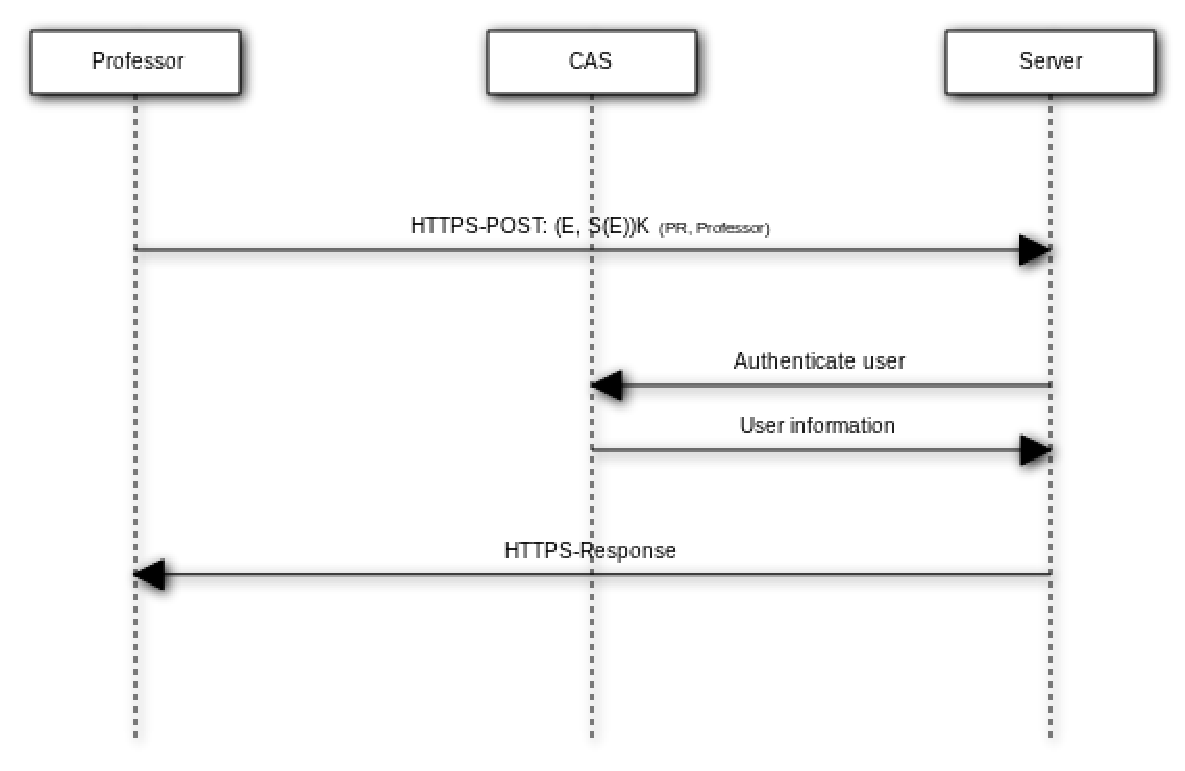
\includegraphics[width=0.75\textwidth]{images/upload_exam.pdf}
\caption{Messages exchanged when uploading an exam}
\label{fig:upload)exam}
\end{center}
\end{figure}

\begin{figure}
\begin{center}
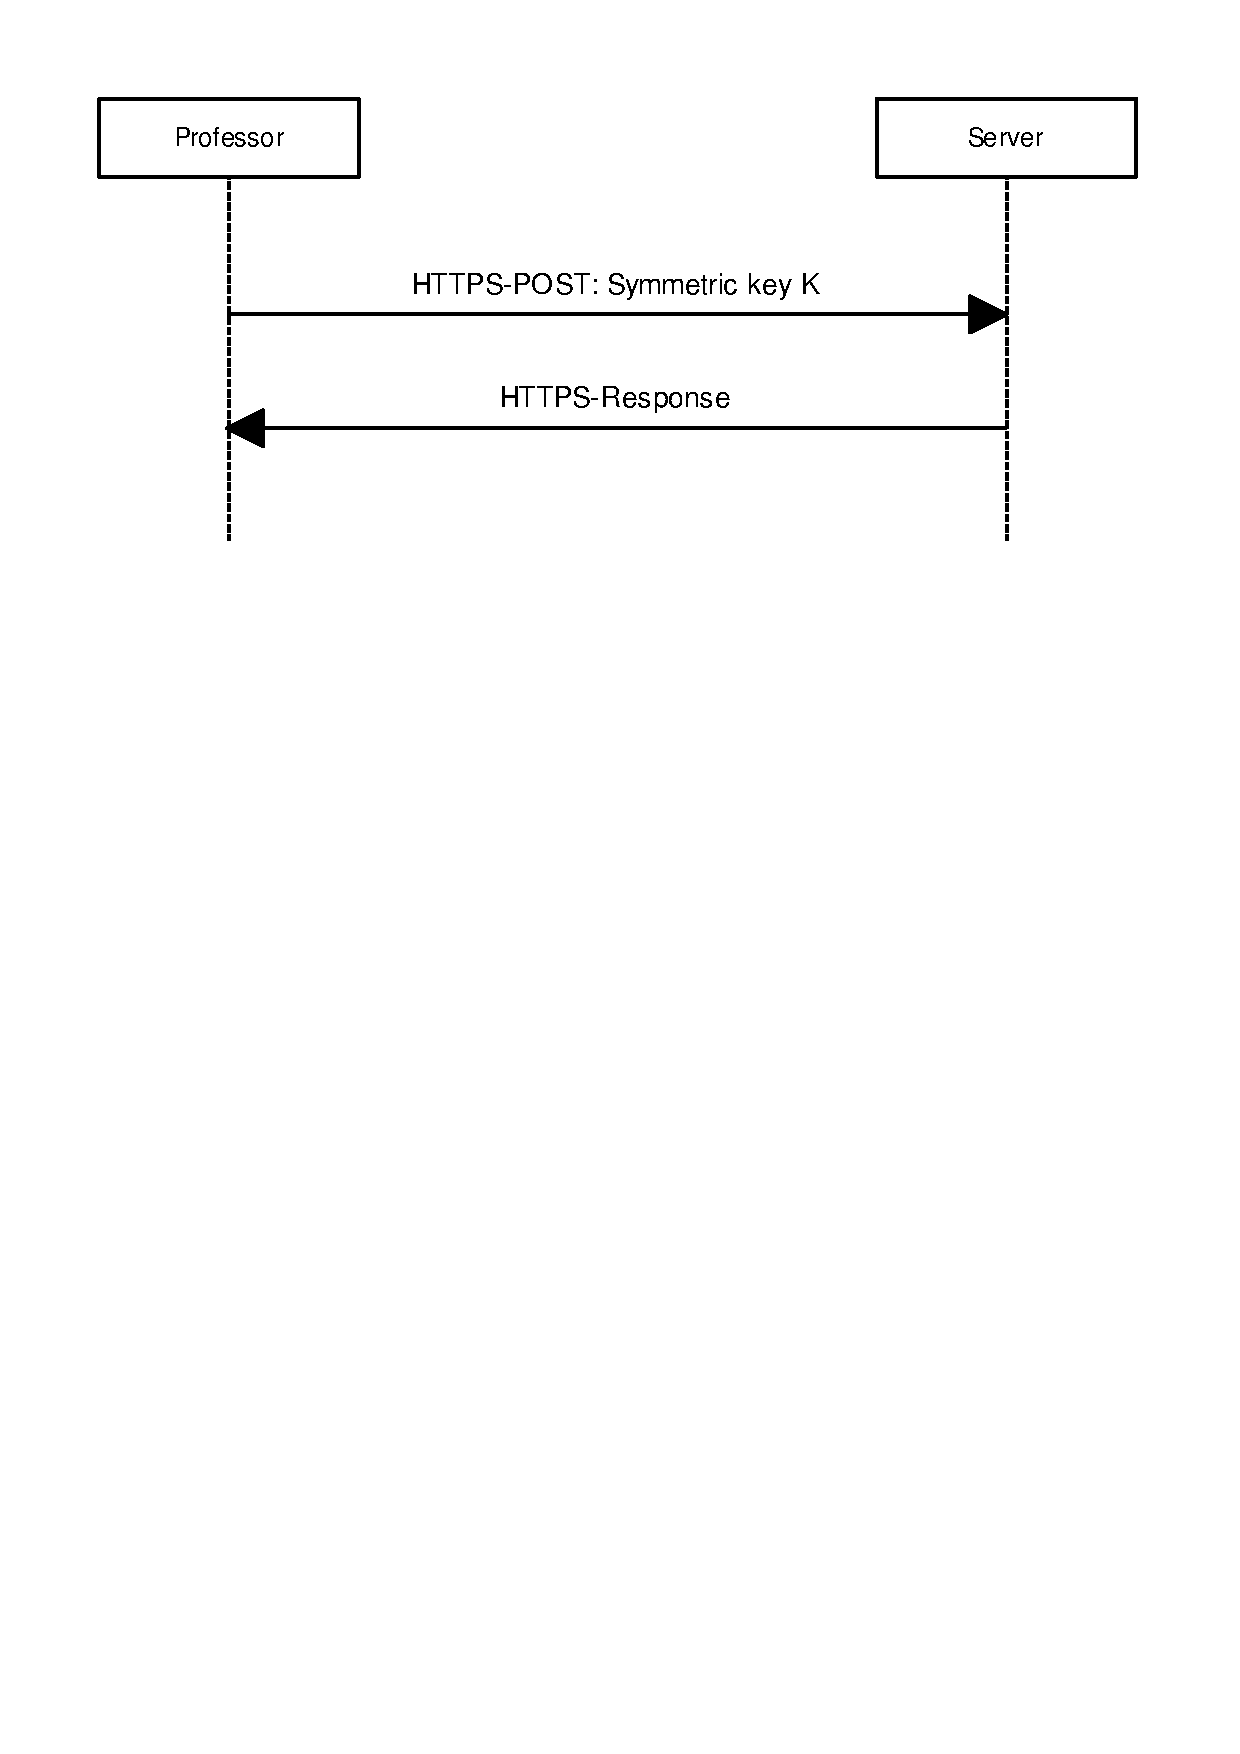
\includegraphics[width=0.75\textwidth]{images/unlock_exam.pdf}
\caption{Messages exchanged when unlocking an exam}
\label{fig:unlock-exam}
\end{center}
\end{figure}

\begin{figure}
\begin{center}
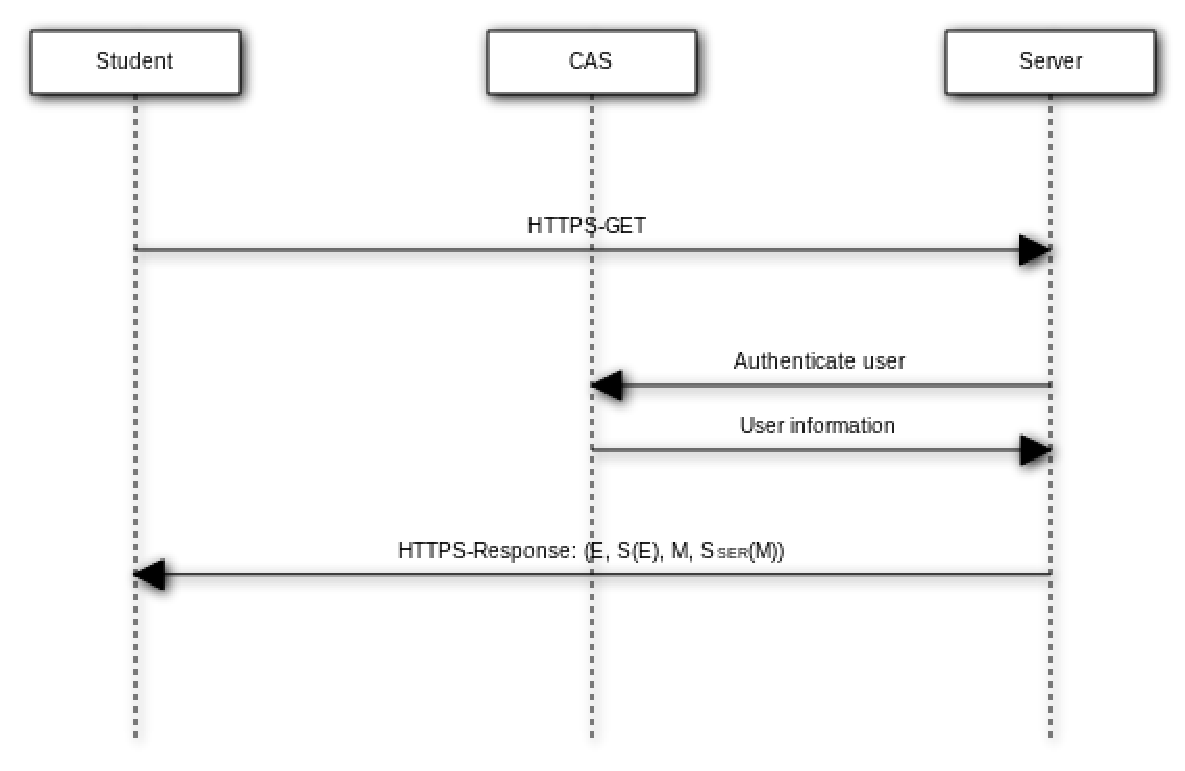
\includegraphics[width=0.75\textwidth]{images/download_exam.pdf}
\caption{Messages exchanged when downloading an exam}
\label{fig:download-exam}
\end{center}
\end{figure}

\begin{figure}
\begin{center}
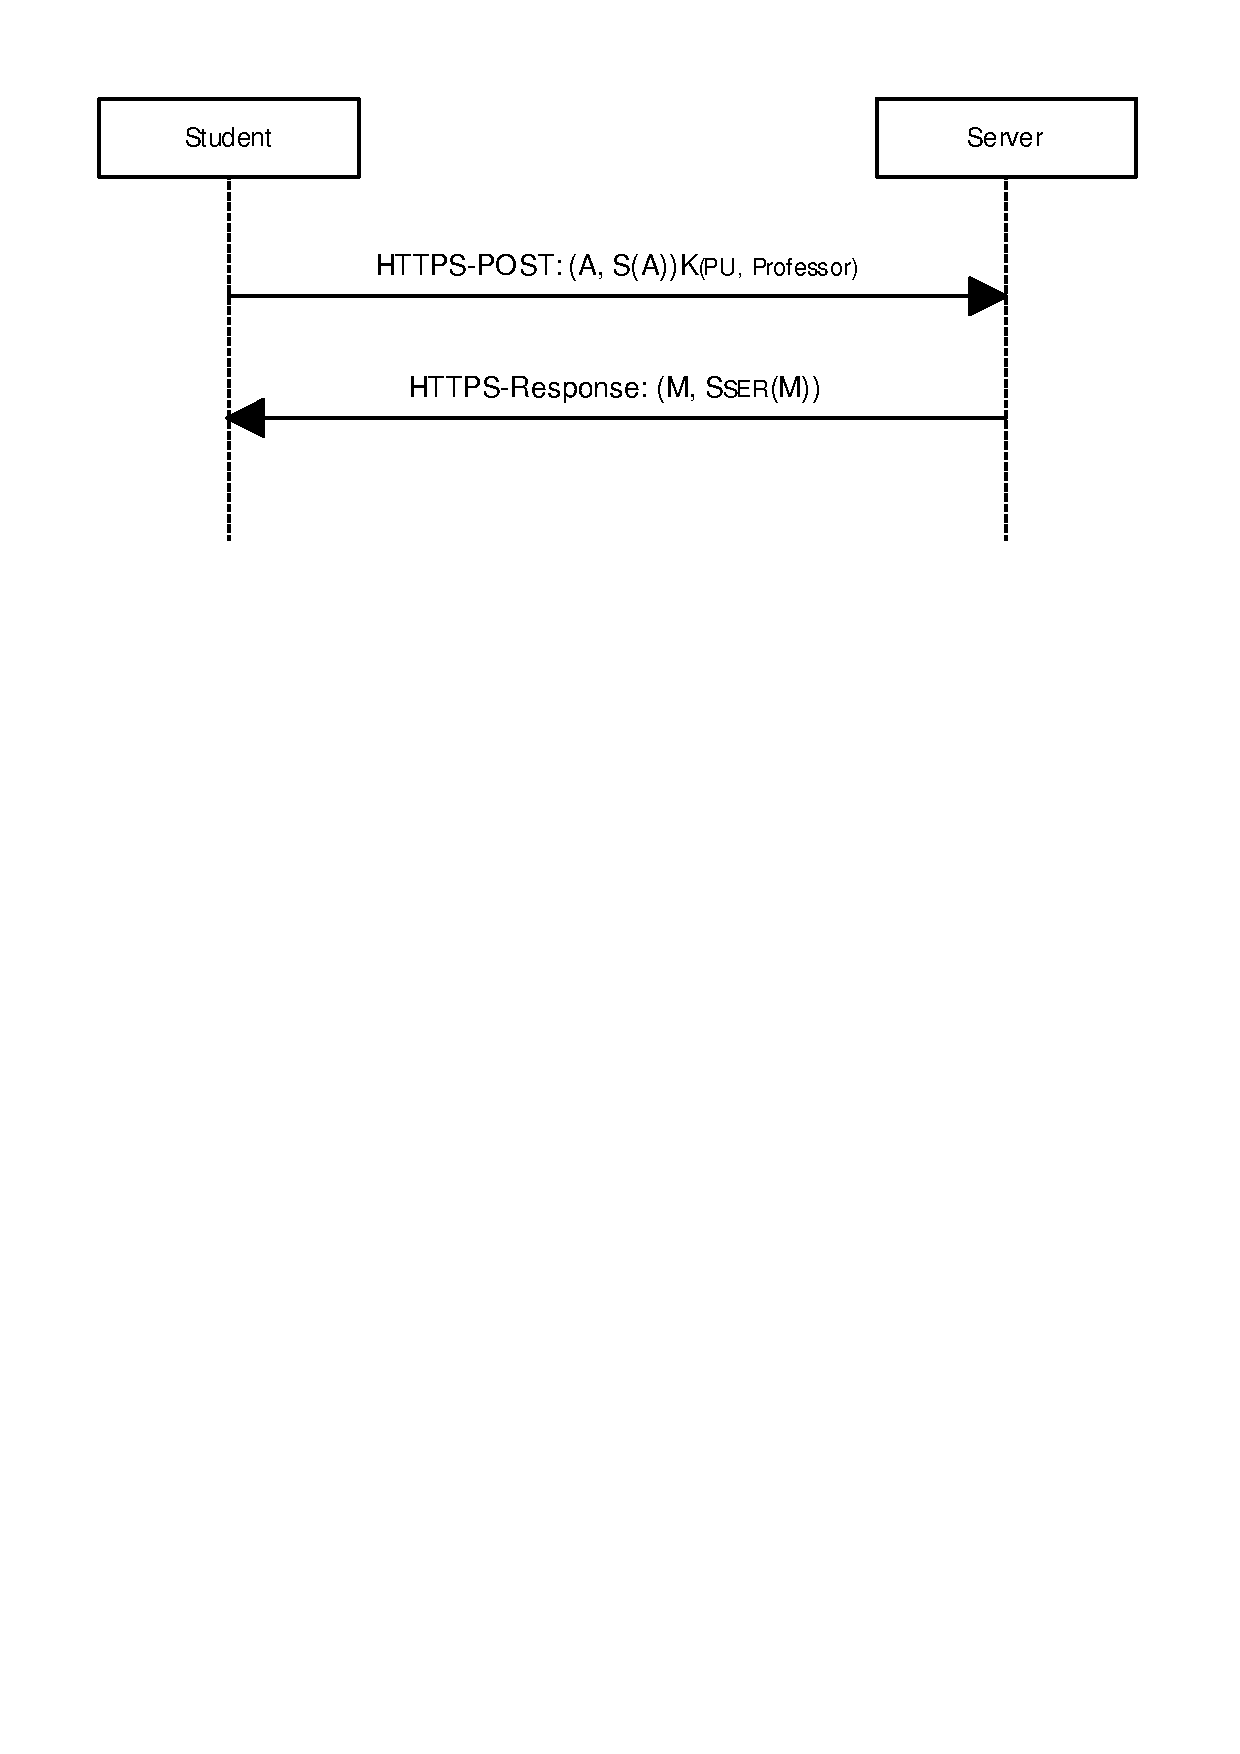
\includegraphics[width=0.75\textwidth]{images/upload_answers.pdf}
\caption{Messages exchanged when uploading answers}
\label{fig:upload-answers}
\end{center}
\end{figure}

\begin{figure}
\begin{center}
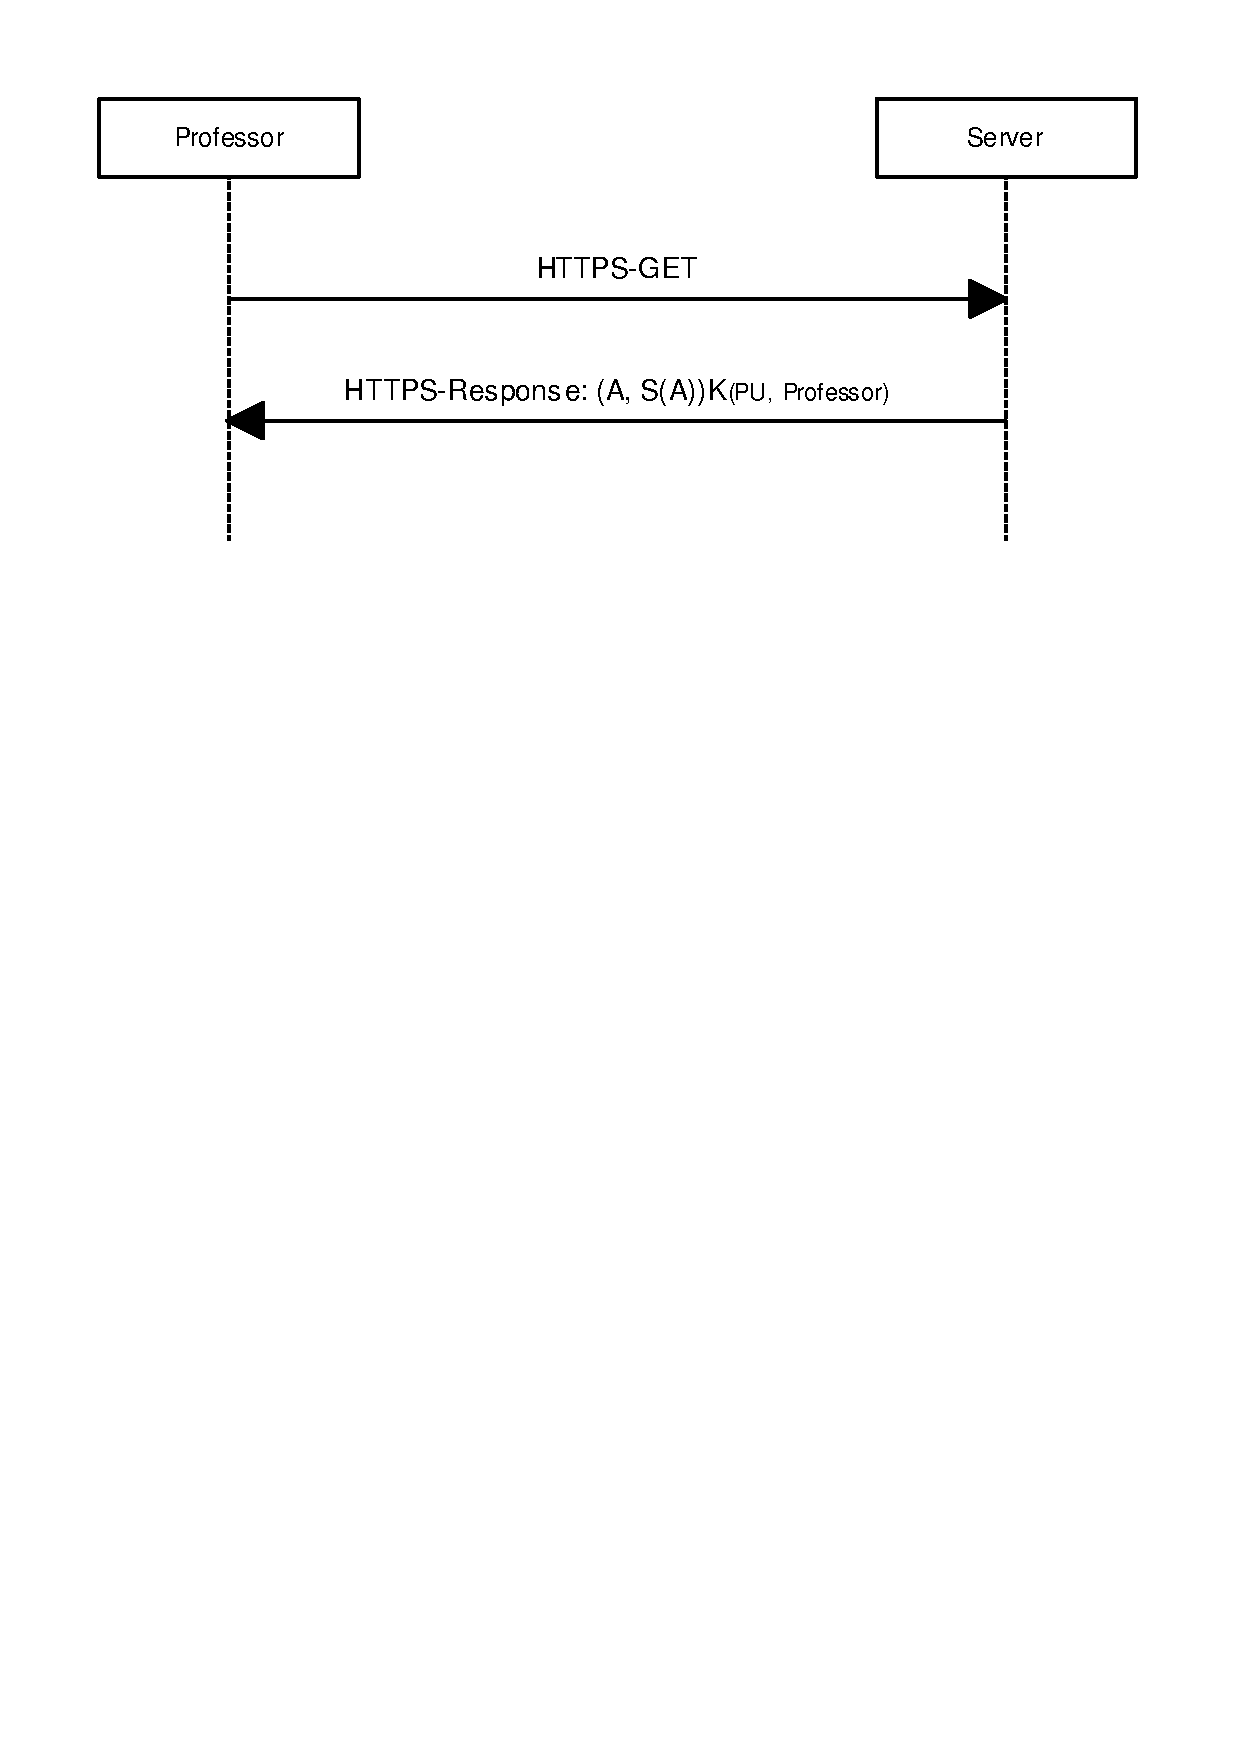
\includegraphics[width=0.75\textwidth]{images/download_answers.pdf}
\caption{Messages exchanged when downloading answers}
\label{fig:download-answers}
\end{center}
\end{figure}

\begin{figure}
\begin{center}
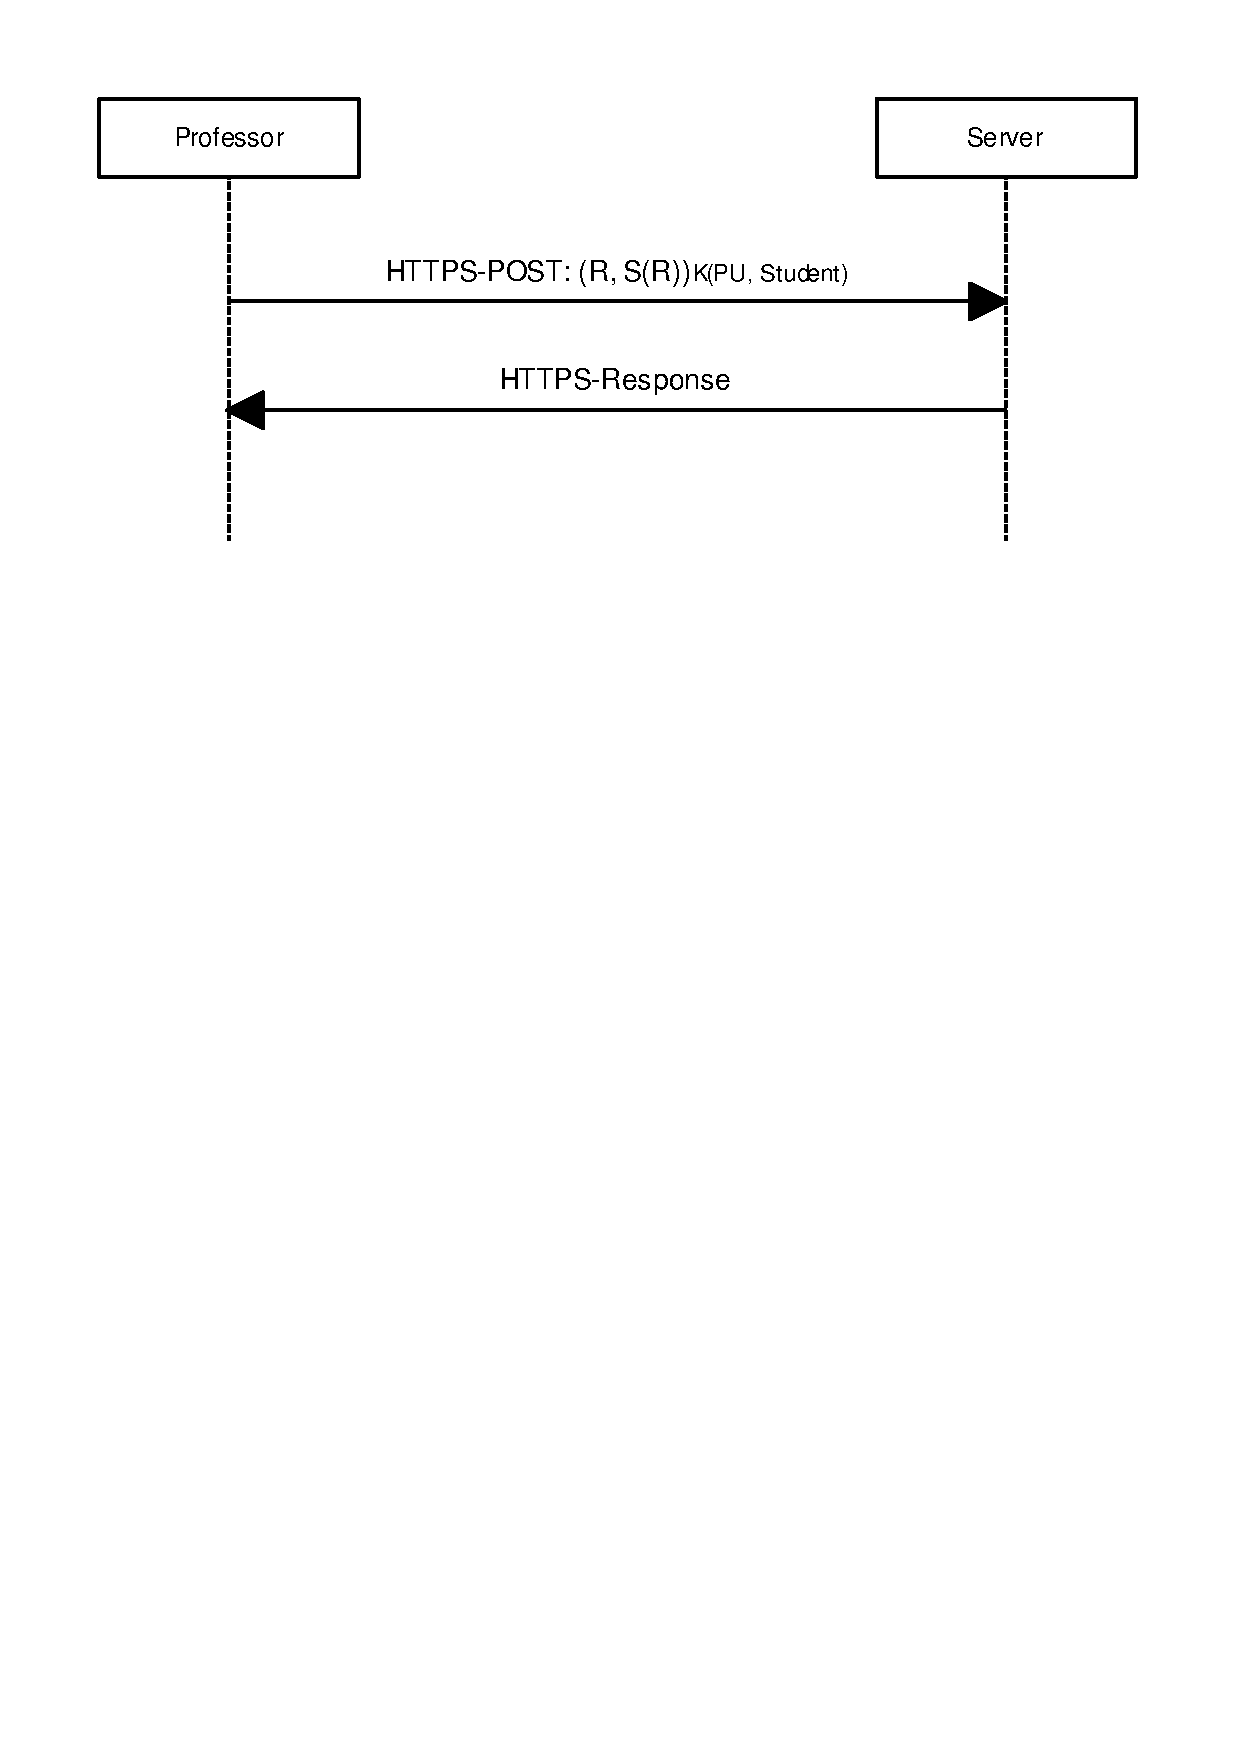
\includegraphics[width=0.75\textwidth]{images/upload_scores.pdf}
\caption{Messages exchanged when uploading scores}
\label{fig:upload-scores}
\end{center}
\end{figure}

\begin{figure}
\begin{center}
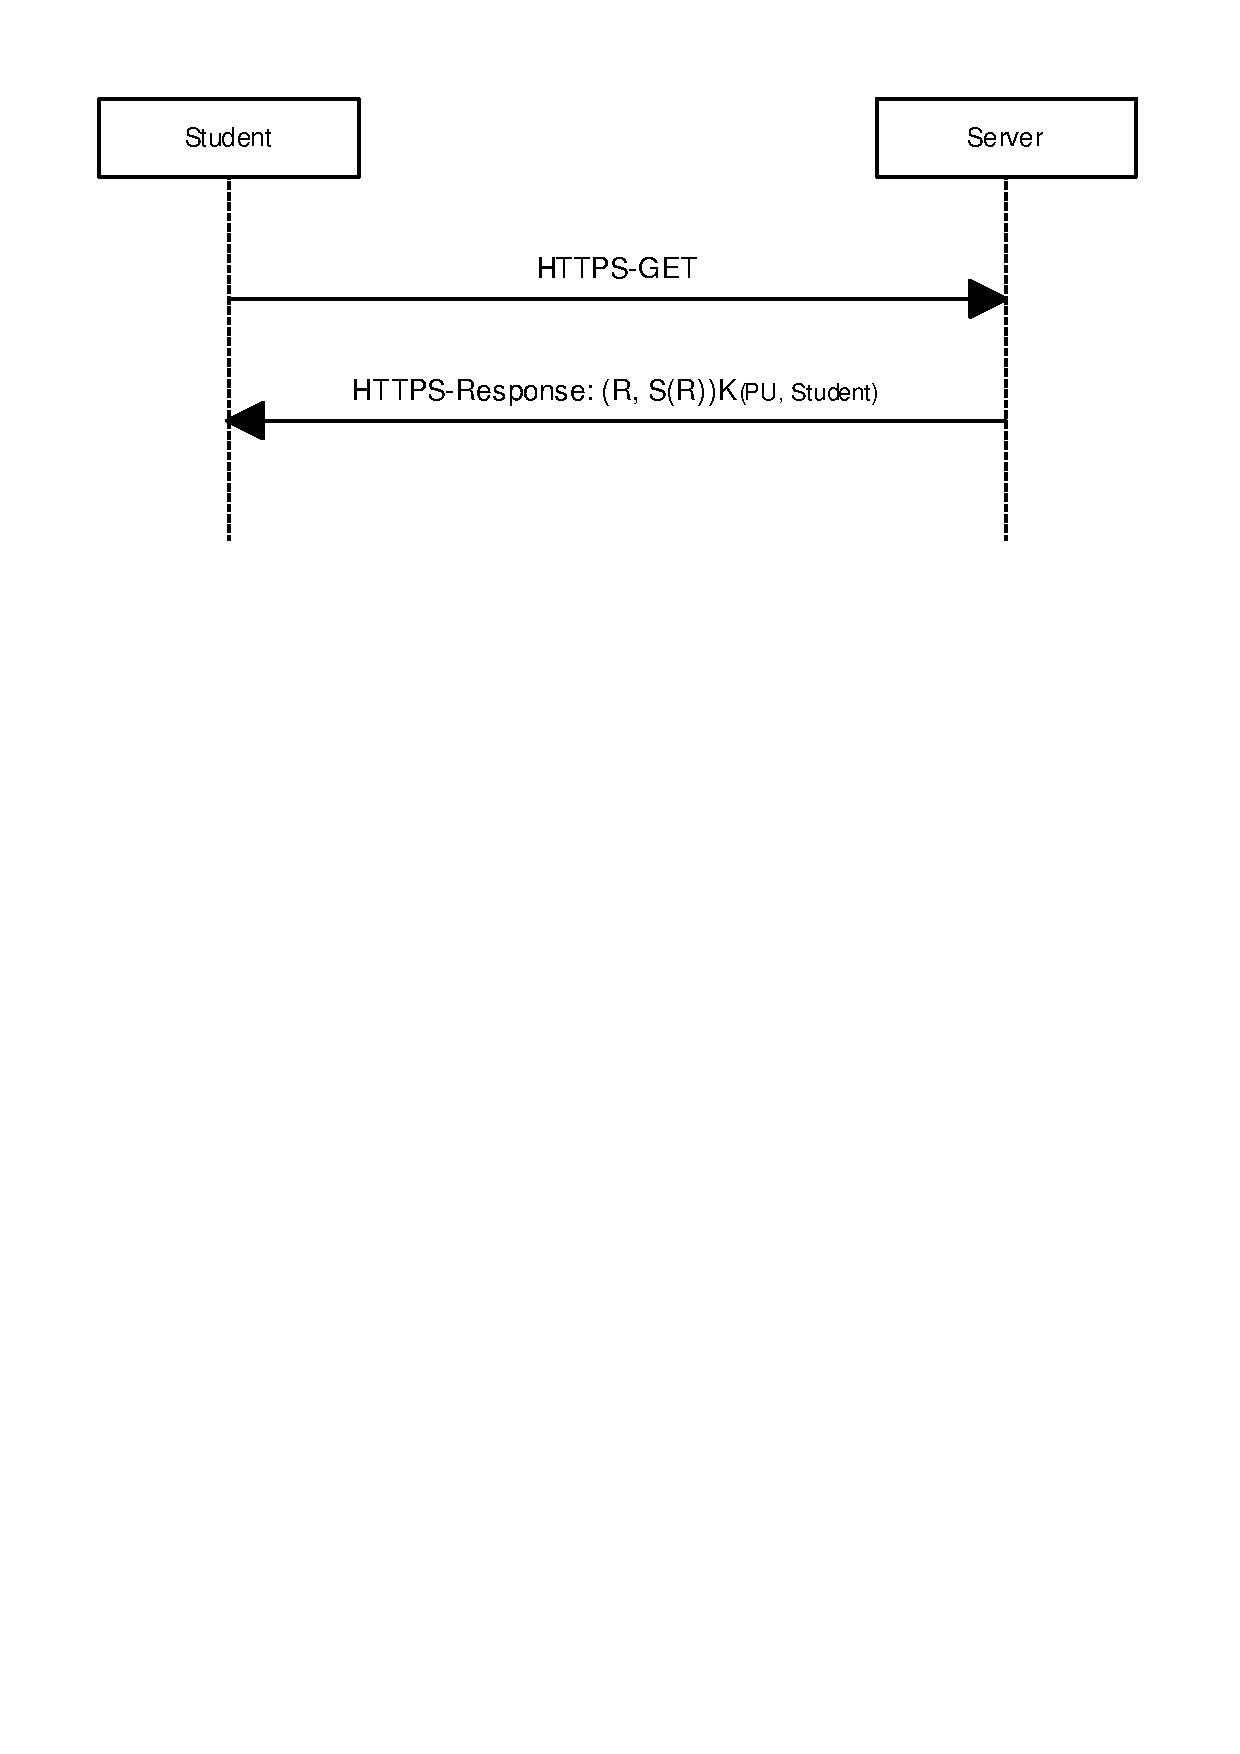
\includegraphics[width=0.75\textwidth]{images/download_scores.pdf}
\caption{Messages exchanged when downloading scores}
\label{fig:download-scores}
\end{center}
\end{figure}

+8000 words.

\end{document}
